\documentclass[11pt,a4paper]{article}

% -------------------- PACKAGES --------------------
\usepackage[utf8]{inputenc}
\usepackage[T1]{fontenc}
\usepackage{lmodern}
\usepackage[a4paper,margin=1in]{geometry}
\usepackage{setspace}
\usepackage{graphicx}
\usepackage{float}
\usepackage{amsmath,amssymb}
\usepackage{booktabs}
\usepackage{array}
\usepackage{tabularx}
\usepackage{xcolor}
\usepackage{hyperref}
\usepackage{xurl}
\usepackage{caption}
\usepackage{enumitem}
\usepackage{microtype}
\usepackage{algorithm}
\usepackage{algpseudocode}
\usepackage{tikz}
\usetikzlibrary{arrows.meta,positioning}
\usepackage{listings}

\onehalfspacing
\setlength{\parindent}{0pt}
\setlength{\parskip}{6pt}
\setcounter{secnumdepth}{3}
\setcounter{tocdepth}{2}
\lstset{basicstyle=\ttfamily\small,breaklines=true,frame=single,columns=fullflexible}

\hypersetup{
    colorlinks=true, linkcolor=black, citecolor=black, urlcolor=blue,
    pdftitle={Final Report: Logit Standardization in Knowledge Distillation},
    pdfauthor={Abiha Jawaid, Bismah Imran, Zainab Asif}
}

% ---------- things the team must still fill in (shown in red; delete when done) ----------
\newcommand{\TODO}[1]{\textcolor{red}{\textbf{[TODO: #1]}}}

% ---------- numbers produced by scripts/make_report_assets.py ----------
\newcommand{\KDacc}{\TODO{KD acc}}
\newcommand{\LSacc}{\TODO{LS acc}}
\newcommand{\CEacc}{\TODO{CE acc}}
\newcommand{\LSgain}{\TODO{gain}}
\newcommand{\CTENkd}{\TODO{C10 KD}}
\newcommand{\CTENls}{\TODO{C10 LS}}
\newcommand{\CTENgain}{\TODO{C10 gain}}
\newcommand{\KDlogitstd}{\TODO{std}}
\newcommand{\LSlogitstd}{\TODO{std}}
\newcommand{\Tlogitstd}{\TODO{std}}
\IfFileExists{generated/numbers.tex}{\renewcommand{\KDacc}{70.92}
\renewcommand{\LSacc}{70.95}
\renewcommand{\CEacc}{69.70}
\renewcommand{\LSgain}{0.03}
\renewcommand{\CTENkd}{93.19}
\renewcommand{\CTENls}{93.11}
\renewcommand{\CTENgain}{-0.08}
\renewcommand{\KDlogitstd}{3.80}
\renewcommand{\LSlogitstd}{1.64}
\renewcommand{\Tlogitstd}{3.90}
}{}

% table bodies from generated/ (or a placeholder row); decided in the preamble so the
% expansion inside tabular stays clean
\makeatletter
\newcommand{\declaretable}[2]{%
  \IfFileExists{generated/#1.tex}%
    {\@namedef{gentab@#1}{\@@input generated/#1.tex }}%
    {\@namedef{gentab@#1}{\multicolumn{#2}{c}{\TODO{run scripts/make\_report\_assets.py}} \\}}}
\newcommand{\gentable}[2]{\csname gentab@#1\endcsname}
\makeatother
\declaretable{tab_repro}{5}
\declaretable{tab_diag}{9}
\declaretable{tab_ablation}{4}
\declaretable{tab_c10}{3}
\declaretable{tab_tau}{3}
\declaretable{tab_runs}{8}

% figure from figures/ (or a given path) or a placeholder box
\newcommand{\maybefig}[4][0.85]{%
\begin{figure}[H]
    \centering
    \IfFileExists{#2}{\includegraphics[width=#1\textwidth]{#2}}{%
        \fbox{\parbox[c][3.5cm][c]{0.8\textwidth}{\centering\textbf{Figure placeholder}\\[4pt]\texttt{\detokenize{#2}}}}}
    \caption{#3}
    \label{#4}
\end{figure}}

\begin{document}

% ==================== TITLE PAGE ====================
\begin{titlepage}
    \centering
    \vspace*{1.2cm}
    {\Large \textbf{FINAL REPORT}\par}
    \vspace{1cm}
    {\LARGE \textbf{Logit Standardization in Knowledge Distillation:\\[4pt]Reproduction, Experiments and Deployment}\par}
    \vspace{1cm}
    {\large Machine Learning -- CSE-602 \quad|\quad Fall 2026\par}
    \vspace{1cm}
    \textbf{Team Members}\\[6pt]
    Abiha Jawaid (36395)\\
    Bismah Imran (36222)\\
    Zainab Asif (36232)
    \vspace{1cm}

    \textbf{Reproduced paper:} S. Sun, W. Ren, J. Li, R. Wang and X. Cao,\\
    ``Logit Standardization in Knowledge Distillation,'' CVPR 2024.
    \vspace{1cm}

    \fbox{\parbox{0.85\textwidth}{\centering
    \textbf{Project artifacts (public, view/download without permission)}\\[4pt]
    Source code: \TODO{GitHub URL}\\
    Trained model weights: \TODO{Google Drive / Hugging Face URL}\\
    Web app: run locally with \texttt{streamlit run app.py} (Section~\ref{sec:deploy})}}
    \vfill
    {\large Submitted: 25 November 2026\par}
\end{titlepage}

\begin{abstract}
Knowledge distillation (KD) trains a small \emph{student} network to imitate the softened class probabilities of a large \emph{teacher}. Sun et al.\ (CVPR 2024) argue that the usual practice of using one shared softmax temperature for teacher and student silently forces the student to reproduce the teacher's logit \emph{scale} (range and variance), even though only the \emph{relations} between class scores are needed. They propose a parameter-free Z-score \emph{logit standardization} (LS) of both logit vectors before the softmax. We re-implemented vanilla KD and KD+LS in PyTorch, distilled a pretrained ResNet-56 teacher into a ResNet-20 student on CIFAR-100, and compared against the paper's reported numbers (KD $70.66\%$, KD+LS $71.43\%$). Our runs give \KDacc\% and \LSacc\% respectively (a gain of \LSgain\ percentage points). Beyond reproduction, we ran (A) a $2\times2$ ablation separating the effect of the Z-score from the ten-times-larger distillation weight that LS uses, and (B) a dataset-variation study on CIFAR-10. Finally, we deployed both students in a Streamlit web application that shows the full inference pipeline and visualises raw versus standardized logits for any uploaded image.
\end{abstract}

\tableofcontents
\newpage

% ============================================================
\section{Introduction and Problem Statement}
% ============================================================

Deep networks with high accuracy are often too large or too slow for phones, embedded devices or high-throughput services. \emph{Knowledge distillation} \cite{hinton2015} is a model-compression technique: a high-capacity \emph{teacher} that has already been trained supervises the training of a compact \emph{student}. Besides the ground-truth label, the student is asked to match the teacher's full probability distribution over classes, which carries ``dark knowledge'' such as \emph{a leopard looks more like a tiger than like a bicycle}.

In standard logit-based KD, both networks' logits are divided by the \emph{same} temperature $T$ before the softmax, and the student minimises the Kullback--Leibler (KL) divergence between the two softened distributions. Sun et al.\ \cite{sun2024} show that this shared temperature has a hidden side-effect: at the optimum, the student's logits must equal the teacher's logits up to a constant shift, and therefore must have the \emph{same standard deviation}. A small student may not be able to produce logits as large and as spread out as a big teacher's, and it does not need to---it only needs the right \emph{ranking and relative spacing} of classes to predict well.

\textbf{Problem statement.} Does removing this implicit ``match the teacher's logit magnitude'' constraint---by Z-score standardizing teacher and student logits separately before the softmax---help a small student learn from a large teacher, and if so, why?

\textbf{Objectives of this project.}
\begin{enumerate}[nosep]
    \item Explain the paper's method and theory in our own words (Section~\ref{sec:method}).
    \item Re-implement vanilla KD and KD+LS and reproduce the paper's ResNet-56$\rightarrow$ResNet-20 CIFAR-100 result (Sections~\ref{sec:impl}--\ref{sec:repro}).
    \item Answer two additional research questions experimentally (Section~\ref{sec:exp}).
    \item Deploy the trained students in a web application (Section~\ref{sec:deploy}).
\end{enumerate}

% ============================================================
\section{Literature Review / Background}
% ============================================================
\emph{(Carried over from the Mid-Evaluation report, lightly refined; see Appendix~\ref{app:revisions}.)}

\subsection{Background and importance}
Deep neural networks achieve strong image-classification results, but high-performing models can require substantial memory, computation and energy, which creates a deployment barrier for devices with limited resources. Model compression seeks to reduce these costs while retaining predictive performance; knowledge distillation is one such approach in which a high-capacity teacher guides a smaller student during training \cite{hu2023,mansourian2025}.

Hinton, Vinyals and Dean formalised the widely used KD formulation in which the student learns from the teacher's softened class-probability distribution as well as from the ground-truth labels \cite{hinton2015}. The teacher's output provides more information than a one-hot label: it expresses that some incorrect classes are more similar to the target than others (``dark knowledge''). The selected CVPR 2024 paper studies one specific issue inside this framework: how teacher and student logits are converted into probability distributions \cite{sun2024}.

\subsection{Conventional knowledge distillation}
For an input image a classifier outputs one real-valued score (\emph{logit}) $z_k$ per class. With temperature $T$ the softmax gives
\begin{equation}
q_k = \frac{\exp(z_k/T)}{\sum_{j}\exp(z_j/T)} .
\label{eq:softmax}
\end{equation}
A larger $T$ flattens the distribution so that the small probabilities of non-target classes become visible to the student. Conventional KD combines a cross-entropy (CE) term with the ground truth and a KL term between teacher and student distributions computed with the \emph{same} $T$ \cite{hinton2015}.

\subsection{Earlier knowledge distillation approaches}
KD methods are commonly grouped by what is transferred: \emph{logit-based} methods use final predictions, \emph{feature-based} methods match intermediate representations, and \emph{relation-based} methods transfer relationships among samples or representations \cite{hu2023,mansourian2025,sun2024}.

\textbf{Logit-based.} Decoupled KD (DKD) splits the loss into target-class and non-target-class parts and weights them separately \cite{zhao2022}. Curriculum Temperature KD (CTKD) learns an adaptive, sample-wise temperature adversarially \cite{li2023}, but still shares it between teacher and student. Multi-Level Logit Distillation (MLKD) aligns predictions at instance, batch and class level \cite{jin2023}. Normalized KD changes the treatment of the non-target part of the output \cite{yang2023}; Scale Decoupled Distillation splits global logits into local ones \cite{wei2024}; and Refined Logit Distillation uses labels to correct misleading teacher logits \cite{sun2025}. ATKD \cite{guo2022} chooses adaptive temperatures to reduce a teacher--student ``sharpness'' gap, but relies on an approximately zero logit mean. None of these questions why teacher and student \emph{share} the temperature---the assumption Sun et al.\ challenge.

\textbf{Feature- and relation-based.} FitNets \cite{romero2015}, attention transfer, CRD \cite{tian2020} and ReviewKD \cite{chen2021} make the student imitate intermediate teacher features, which gives richer supervision but needs extra projection layers and depends on the two architectures. Relation-based methods such as RKD \cite{park2019} transfer distances or angles between samples. These are generally stronger than vanilla KD but more complex; LS is attractive because it brings plain logit KD close to them with \emph{no} extra parameters.

\textbf{Capacity gap.} Several works observe that a larger teacher is not always a better teacher for a small student \cite{cho2019,mirzadeh2020}. Sun et al.\ offer a new explanation: a small student cannot reproduce the compact, large-range logits of a big teacher, and shared-temperature KD asks it to.

\subsection{Research gap and project scope}
The paper establishes LS as a lightweight way to relax the shared-scale constraint and reports results averaged over four runs on many teacher--student pairs. Our project (i) reproduces the ResNet-56$\rightarrow$ResNet-20 CIFAR-100 pair with our own implementation; (ii) tests whether the improvement is really caused by the standardization or by the much larger distillation weight that the LS recipe uses---a confound that matters for anyone adopting the method; and (iii) tests our own hypothesis that, because the mean and standard deviation are estimated from only $K$ logits per image, the benefit may differ when there are only $K{=}10$ classes (CIFAR-10).

% ============================================================
\section{Paper Methodology}
\label{sec:method}
% ============================================================

\subsection{Notation}
For image $x_n$ the teacher outputs logits $\mathbf{v}_n\in\mathbb{R}^K$ and the student $\mathbf{z}_n\in\mathbb{R}^K$, with $K$ classes. Vanilla KD minimises
\begin{equation}
\mathcal{L} = \lambda_{CE}\,\mathrm{CE}\big(y_n,\mathrm{softmax}(\mathbf{z}_n)\big) + \lambda_{KD}\,T^2\,\mathrm{KL}\big(\mathrm{softmax}(\mathbf{v}_n/T)\,\|\,\mathrm{softmax}(\mathbf{z}_n/T)\big).
\label{eq:kd}
\end{equation}
The factor $T^2$ keeps the gradient size roughly independent of $T$, because the gradient of the softened KL shrinks like $1/T^2$ \cite{hinton2015}.

\subsection{Where does the temperature come from? (entropy maximisation)}
The authors show that the softmax itself can be derived as the solution of a constrained optimisation: find the probability vector with the \emph{maximum entropy} (the least committed distribution) subject to (a) the probabilities summing to one and (b) the expected logit being equal to the logit of the correct class. Solving with Lagrange multipliers gives $q^{(k)}\propto\exp(\alpha\,v^{(k)})$, i.e.\ exactly a softmax, where the multiplier $\alpha$ plays the role of $1/T$. Doing the same for the student (with an extra constraint tying it to the teacher) gives $q^{(k)}\propto\exp(\beta\,z^{(k)})$ with its own multiplier $\beta$.

The key observation is that nothing in either derivation forces $\alpha=\beta$, nor forces them to be the same for every image. In other words, \emph{the theory allows the teacher and the student to have different temperatures, and each sample to have its own}. Sharing one global $T$ is a convention, not a requirement.

\subsection{Two side-effects of a shared temperature}
Write each softmax with a general shift $a$ and scale $b$: $q^{(k)}\propto\exp\big((z^{(k)}-a)/b\big)$. If the student is perfectly distilled, its probabilities equal the teacher's for every class. Taking the ratio of any two classes $i,j$ and then averaging over $j$ gives
\begin{equation}
\frac{z^{(i)}-\bar z}{b_S}=\frac{v^{(i)}-\bar v}{b_T},
\qquad\text{and therefore}\qquad
\frac{\sigma(\mathbf{z})}{\sigma(\mathbf{v})}=\frac{b_S}{b_T}.
\label{eq:shackles}
\end{equation}
With a shared temperature ($b_S=b_T$) this yields two ``shackles'':
\begin{enumerate}[nosep]
\item \textbf{Logit shift:} $z^{(i)}=v^{(i)}+\Delta$ --- the student must copy the teacher's logits exactly up to one constant.
\item \textbf{Variance match:} $\sigma(\mathbf{z})=\sigma(\mathbf{v})$ --- the student's logits must be exactly as spread out as the teacher's.
\end{enumerate}
But for correct prediction it is enough that the student \emph{ranks} the classes like the teacher \cite{huang2022}. Forcing a small network to also match the scale wastes capacity and, as the paper's Fig.~3 shows, a vanilla-KD student often cannot reach the teacher's target logit (7.5 vs.\ 12 in their example).

\subsection{The proposed fix: Z-score logit standardization}
Choose each model's ``temperature'' adaptively as the standard deviation of its own logits (times a shared base temperature $\tau$), and subtract each model's own mean:
\begin{equation}
\mathcal{Z}(\mathbf{z};\tau)=\frac{\mathbf{z}-\bar{z}}{\sigma(\mathbf{z})\,\tau},\qquad
\bar z=\frac1K\sum_k z^{(k)},\quad
\sigma(\mathbf{z})=\sqrt{\tfrac1K\textstyle\sum_k (z^{(k)}-\bar z)^2}.
\label{eq:zscore}
\end{equation}
The distillation term becomes $\tau^2\,\mathrm{KL}\big(\mathrm{softmax}(\mathcal{Z}(\mathbf{v};\tau))\,\|\,\mathrm{softmax}(\mathcal{Z}(\mathbf{z};\tau))\big)$, while the CE term still uses the raw student logits. Because $b_S\propto\sigma(\mathbf{z})$ and $b_T\propto\sigma(\mathbf{v})$, Eq.~\eqref{eq:shackles} is now satisfied automatically for \emph{any} student scale. The Z-score has four useful properties:
\begin{itemize}[nosep]
\item \textbf{Zero mean} -- guaranteed exactly (previous work only assumed it).
\item \textbf{Fixed standard deviation} $1/\tau$ -- teacher and student are mapped to the same scale; the student's original scale is free.
\item \textbf{Monotonicity} -- it is a positive linear map, so the class ranking is unchanged and the ``innate relations'' are preserved.
\item \textbf{Boundedness} -- standardized values lie in $[-\sqrt{K-1}/\tau,\sqrt{K-1}/\tau]$, avoiding huge exponentials.
\end{itemize}
A direct consequence (which we verify in our unit tests): if the student's logits are \emph{any} positive affine transform of the teacher's, $\mathbf{z}=a\mathbf{v}+b$ with $a>0$, the LS loss is exactly zero, whereas the vanilla KD loss is not.

Note that only the division by $\sigma$ matters for the loss: the softmax is invariant to adding a constant, so subtracting the mean alone changes nothing (also verified in our tests, and visible in the paper's ablation where ``$z-\bar z$'' performs like vanilla KD).

\begin{algorithm}[H]
\caption{KD with logit standardization (paper Algorithm 2, as implemented in \texttt{lskd/losses.py})}
\begin{algorithmic}[1]
\For{each mini-batch $(x,y)$}
  \State $\mathbf{v}\gets f_T(x)$ \Comment{frozen teacher, no gradient}
  \State $\mathbf{z}\gets f_S(x)$
  \State $p_T\gets\mathrm{softmax}(\mathcal{Z}(\mathbf{v};\tau))$, \quad $p_S\gets\mathrm{softmax}(\mathcal{Z}(\mathbf{z};\tau))$
  \State $\mathcal{L}\gets\lambda_{CE}\,\mathrm{CE}(y,\mathrm{softmax}(\mathbf{z}))+\lambda_{KD}\,\tau^2\,\mathrm{KL}(p_T\|p_S)$
  \State update $f_S$ by SGD on $\mathcal{L}$
\EndFor
\end{algorithmic}
\end{algorithm}

\subsection{Toy example (re-computed by us)}
The paper's Fig.~2 illustrates that vanilla KL can rank students wrongly. We re-computed it with \texttt{scripts/toy\_example.py} (classes cat, dog, bird, frog; $T=\tau=1$) and obtained exactly the paper's numbers (Table~\ref{tab:toy}). Student~S1 is ``closer'' to the teacher in raw magnitude and gets the lower vanilla loss, yet predicts the wrong class; student~S2 is the teacher scaled by $1/10$, predicts correctly and, after standardization, has zero loss.

\begin{table}[H]
\centering
\caption{Toy example of Sun et al.\ (Fig.~2), recomputed by our script. Logits are (cat, dog, bird, frog).}
\label{tab:toy}
\begin{tabular}{lcccc}
\toprule
 & Logits & Prediction & Vanilla KL & KL after Z-score \\
\midrule
Teacher & (1.0, 4.0, 3.0, 2.0) & dog & -- & -- \\
Student S1 & (1.0, 2.8, 3.0, 2.0) & bird (wrong) & \textbf{0.1749} & 0.0995 \\
Student S2 & (0.1, 0.4, 0.3, 0.2) & dog (correct) & 0.3457 & \textbf{0.0000} \\
\bottomrule
\end{tabular}
\end{table}

\subsection{Loss weights}
Because LS lets the student focus on the teacher's relations rather than on hard labels, and because standardization shrinks gradients by $1/\sigma$, the authors use a much larger KD weight with LS ($\lambda_{CE}=0.1$, $\lambda_{KD}=9$, $\tau=2$) than vanilla KD ($\lambda_{CE}=0.1$, $\lambda_{KD}=0.9$, $T=4$). Their ablation (Table~4) shows that vanilla KD collapses when $\lambda_{KD}$ grows (73.33\% at $\lambda_{KD}=9$, 63.45\% at 18 for ResNet32$\times$4$\rightarrow$ResNet8$\times$4), while LS stays stable. This difference in weights is the confound our Experiment~A investigates.

\subsection{Datasets, metrics and the paper's findings}
The paper evaluates on CIFAR-100 and ImageNet with top-1 (and top-5 on ImageNet) accuracy, averaging four runs. LS improves every logit-based method it is added to (KD, CTKD, DKD, MLKD). For our pair, ResNet-56 (72.34\%)$\rightarrow$ResNet-20 (69.06\% alone), the paper reports 70.66\% for KD and 71.43\% for KD+LS (+0.77). LS-distilled students also show better-separated t-SNE features, logits whose \emph{standardized} values match the teacher closely while their raw scale is free, and consistent gains across teachers of different size.

% ============================================================
\section{Implementation Details}
\label{sec:impl}
% ============================================================

\subsection{Architectures}
Both networks are CIFAR-style ResNets \cite{he2016}: a $3{\times}3$ convolution with 16 filters, three stages of $n$ residual BasicBlocks with 16, 32 and 64 filters (stages 2 and 3 halve the resolution $32\to16\to8$), global average pooling and a linear layer; depth $=6n+2$.

\begin{table}[H]
\centering
\caption{Teacher and student networks (parameter counts from our code, 100 classes).}
\label{tab:arch}
\begin{tabular}{lcccc}
\toprule
Model & Depth & Blocks per stage & Parameters & Role \\
\midrule
ResNet-56 & 56 & 9 & 0.862 M & teacher (frozen, pretrained) \\
ResNet-20 & 20 & 3 & 0.278 M & student (trained) \\
\bottomrule
\end{tabular}
\end{table}

\subsection{Training configuration}
We follow the paper/mdistiller CIFAR-100 recipe (Table~\ref{tab:hparams}). Each run is a named preset in \texttt{lskd/experiments.py}.

\begin{table}[H]
\centering
\caption{Training hyper-parameters (identical for all runs unless stated).}
\label{tab:hparams}
\begin{tabular}{ll}
\toprule
Optimizer & SGD, momentum 0.9, weight decay $5\times10^{-4}$ \\
Batch size / epochs & 64 / 240 \\
Learning rate & 0.05, multiplied by 0.1 at epochs 150, 180, 210 \\
Augmentation (train only) & random $32{\times}32$ crop from 4-px zero padding, horizontal flip \\
Vanilla KD & $T=4$, $\lambda_{CE}=0.1$, $\lambda_{KD}=0.9$ \\
KD + LS & $\tau=2$, $\lambda_{CE}=0.1$, $\lambda_{KD}=9$ \\
Teacher & ResNet-56 pretrained (72.34\%), eval mode, no gradients \\
Seed & 0 (one run per configuration) \\
\bottomrule
\end{tabular}
\end{table}

\subsection{Environment and dependencies}
Training: \TODO{Google Colab / Kaggle}, NVIDIA \TODO{T4/P100} GPU, Python \TODO{3.x}, PyTorch \TODO{2.x} (versions are stored in each run's \texttt{summary.json}). Deployment: a CPU laptop, Python 3.9, PyTorch, torchvision, NumPy, Pillow, Matplotlib, Streamlit (\texttt{requirements.txt}).

\subsection{Code structure}
\begin{itemize}[nosep]
\item \texttt{lskd/losses.py}: \texttt{zscore}, vanilla KD loss, KD+LS loss, total loss (Algorithm~1).
\item \texttt{lskd/models.py}: CIFAR ResNets; \texttt{lskd/data.py}: loading, augmentation, normalization.
\item \texttt{train.py}: training with per-epoch checkpoints, \texttt{--resume} (for cloud disconnects) and \texttt{--smoke} (1-minute pipeline check).
\item \texttt{evaluate.py}: accuracy, calibration, logit statistics and teacher-agreement diagnostics.
\item \texttt{infer.py}, \texttt{lskd/inference.py}, \texttt{app.py}: inference and deployment.
\item \texttt{scripts/make\_report\_assets.py}: generates every table and figure of Sections 6--7 from the run logs, so the report numbers cannot drift from the logs.
\item \texttt{tests/test\_core.py}: unit tests of the mathematical properties in Section~\ref{sec:method}.
\end{itemize}

\subsection{Code and result attribution}
\begin{table}[H]
\centering
\caption{What we wrote, adapted and reused.}
\label{tab:attr}
\small
\begin{tabularx}{\textwidth}{lXl}
\toprule
Component & Status & Source \\
\midrule
Z-score, KD and KD+LS losses & Implemented by us from the paper's equations; checked against the official \texttt{normalize()} & \cite{sun2024code} \\
CIFAR ResNet definition & Adapted: rewritten, but layer names follow mdistiller so the official teacher checkpoint loads & \cite{mdistiller} \\
ResNet-56 CIFAR-100 teacher weights & Reused (pretrained checkpoint) & \cite{mdistiller} \\
Hyper-parameter values & Reused from paper / official configs & \cite{sun2024} \\
Data pipeline, training, evaluation, inference, web app, report scripts, tests & Implemented by us & -- \\
CIFAR download/parsing & Reused library (\texttt{torchvision}) & -- \\
All students and the CIFAR-10 teacher & Trained by us & -- \\
\midrule
Numbers labelled ``Paper'' & Reported by Sun et al.\ (Table~2) & \cite{sun2024} \\
Numbers labelled ``Ours'' & Obtained by our team & this report \\
\bottomrule
\end{tabularx}
\end{table}
We did not clone and run the official repository; it was used only as a reference to confirm implementation details. AI coding assistants were used while writing parts of the code and text; all components were run, tested and checked by the team (Appendix~\ref{app:ai}).

\subsection{Deviations and feasibility adjustments}
\begin{itemize}[nosep]
\item \textbf{One seed} per configuration instead of the paper's average of four (compute budget). Differences below roughly $\pm0.3$ pp should be treated as within run-to-run noise.
\item \textbf{Mixed precision} (fp16 autocast) for speed on free GPUs; the losses are computed in fp32.
\item \textbf{GPU-side augmentation}: the same crop+flip recipe, executed on the GPU instead of CPU workers.
\item \textbf{Reported metric}: we report the \emph{final-epoch} test accuracy, which does not use the test set for model selection; the mdistiller code family logs the \emph{best} test accuracy over epochs, so we also list best-epoch accuracy for a like-for-like comparison.
\item \textbf{Standard deviation}: as in the official code, $\sigma$ uses the unbiased estimator ($1/(K{-}1)$); the paper's Algorithm~1 writes $1/K$. The two differ by a constant factor $\sqrt{K/(K-1)}$ (1.005 for $K{=}100$), which is equivalent to a 0.5\% change of $\tau$. (The paper's own Fig.~2 values also correspond to the unbiased version.)
\item \TODO{If you trained with fewer than 240 epochs, state it here; it must be the same for all compared runs.}
\end{itemize}

\subsection{Verification of the implementation}
Before training, we checked the implementation with unit tests (\texttt{tests/test\_core.py}): standardized logits have zero mean, unit standard deviation and unchanged class ranking; the LS loss is zero for any student $\mathbf{z}=a\mathbf{v}+b$ ($a>0$) while vanilla KD is not; mean-subtraction alone leaves the KD loss unchanged; network output shapes and parameter counts match Table~\ref{tab:arch}; and the toy example of Table~\ref{tab:toy} matches the paper to four decimals. The loaded teacher reaches \TODO{72.3x}\% on the CIFAR-100 test set with our evaluation code, confirming that weights and preprocessing are consistent with the original.

% ============================================================
\section{Dataset and Preprocessing / EDA}
% ============================================================
\emph{(Carried over from the Mid-Evaluation report; the preprocessing subsection is updated to the final training pipeline.)}

\subsection{Dataset selection and structure}
CIFAR-100 \cite{krizhevsky2009} is the primary dataset because it is used in the paper. It contains 60,000 colour images of $32\times32$ pixels split into 50,000 training and 10,000 test images across 100 classes (grouped into 20 super-classes). CIFAR-10, with the same image format but only 10 classes, is used for Experiment~B. Because the class sets differ, accuracies on the two datasets are reported separately and are not compared directly as measures of method quality.

\begin{table}[H]
\centering
\caption{Dataset statistics (verified in the EDA notebook).}
\label{tab:dataset_statistics}
\begin{tabular}{lrrr}
\toprule
Dataset / split & Images & Classes & Images per class \\
\midrule
CIFAR-100 training & 50,000 & 100 & 500 \\
CIFAR-100 test & 10,000 & 100 & 100 \\
CIFAR-10 training & 50,000 & 10 & 5,000 \\
CIFAR-10 test & 10,000 & 10 & 1,000 \\
\bottomrule
\end{tabular}
\end{table}

\subsection{Class distribution}
The EDA notebook counts labels per split and confirms that every CIFAR-100 class has exactly 500 training and 100 test images (min = max), so overall accuracy is not dominated by any class.

\maybefig[0.6]{Picture1.png}{CIFAR-100 images per class in the official training and test splits.}{fig:classcounts}

\subsection{Raw image inspection}
Each sample is a low-resolution RGB image. At $32\times32$ objects may occupy only part of the image and fine details are ambiguous; several classes are visually similar (e.g.\ maple/oak/willow tree, boy/girl/baby/man/woman), which makes 100-way classification hard.

\maybefig[0.6]{Raw Pictures in CIFAR.png}{Representative raw CIFAR-100 training images and their labels.}{fig:raw}

\subsection{Missing data, anomalies and challenges}
CIFAR is distributed as fixed-size uint8 arrays with integer labels, so missing values are not expected; the notebook nevertheless checks array shape $(50000,32,32,3)$, dtype uint8, pixel range 0--255, finite values and label range 0--99, and all checks pass. The main challenges are low resolution, visually similar fine classes, intra-class variation and run-to-run variance of training.

\subsection{Preprocessing (final pipeline)}
\begin{enumerate}[nosep]
\item uint8 pixels are scaled to $[0,1]$.
\item \textbf{Training only:} the image is zero-padded by 4 pixels and a random $32\times32$ crop is taken, then flipped horizontally with probability 0.5. This is the augmentation used by the paper's code family; it was disabled in the Mid-report notebook only to keep the EDA easy to interpret.
\item Per-channel normalization $x'_c=(x_c-\mu_c)/\sigma_c$ with the CIFAR-100 training statistics $\boldsymbol\mu=(0.5071,0.4867,0.4408)$, $\boldsymbol\sigma=(0.2675,0.2565,0.2761)$ (CIFAR-10: $(0.4914,0.4822,0.4465)$, $(0.2470,0.2435,0.2616)$).
\end{enumerate}
The test set and the deployed app use steps 1 and 3 only, so evaluation is deterministic. No resizing is needed for CIFAR; the app resizes arbitrary uploads to $32\times32$.

\subsection{Evaluation metrics}
Top-1 test accuracy is the primary metric (single-label task, balanced classes), plus top-5 accuracy. As diagnostics we report expected calibration error (ECE, 15 bins), the average per-image standard deviation of the logits, top-1 agreement with the teacher, the Spearman rank correlation between student and teacher logits (how well the class \emph{ranking} is copied), and the KL divergence to the teacher measured both on raw and on standardized logits. Training losses are tracked but, following the paper's argument, not interpreted on their own.

% ============================================================
\section{Reproduction Results}
\label{sec:repro}
% ============================================================

Table~\ref{tab:repro} compares our results with the paper for ResNet-56$\rightarrow$ResNet-20 on CIFAR-100. ``Paper'' numbers are copied from Sun et al.\ (Table~2, mean of 4 runs); ``Ours'' are our single-seed runs.

\begin{table}[H]
\centering
\caption{Reproduction on CIFAR-100 (top-1 \%). Final = last epoch (our primary metric); Best = best epoch (the paper's code-base convention).}
\label{tab:repro}
\begin{tabular}{lcccc}
\toprule
Method & Paper & Ours (final) & Ours (best) & Ours$-$Paper \\
\midrule
\gentable{tab_repro}{5}
\bottomrule
\end{tabular}
\end{table}

\maybefig{figures/curves_c100.pdf}{Test accuracy (left) and unweighted training cross-entropy (right) per epoch for the CIFAR-100 runs. The jumps at epochs 150/180/210 are the learning-rate decays.}{fig:curves}

\begin{table}[H]
\centering
\caption{Diagnostics on the CIFAR-100 test set (\texttt{evaluate.py}). Agree = top-1 agreement with teacher; $\rho$ = mean Spearman correlation of the 100 logits with the teacher's; KL measured with raw logits ($T{=}4$) and with Z-scored logits ($\tau{=}2$).}
\label{tab:diag}
\small
\begin{tabular}{lcccccccc}
\toprule
Model & Top-1 & Top-5 & ECE & Logit std & Agree & $\rho$ & KL raw & KL Z \\
\midrule
\gentable{tab_diag}{9}
\bottomrule
\end{tabular}
\end{table}

\maybefig{figures/logit_stats.pdf}{Distribution over test images of the logit standard deviation (left) and of the gap between the top logit and the mean (right) for the teacher and both students.}{fig:logits}

\TODO{2--4 sentences describing the reproduction result: KD vs paper, KD+LS vs paper, whether the sign and size of the gain match. Example: ``Our vanilla KD student reaches \KDacc\%, X pp from the paper; KD+LS reaches \LSacc\%, so LS improves KD by \LSgain\ pp versus 0.77 pp in the paper.''}

% ============================================================
\section{Additional Experiments}
\label{sec:exp}
% ============================================================

\subsection{Experiment A -- Ablation: is the gain caused by the Z-score or by the larger KD weight?}
\textbf{Research question.} The LS recipe changes two things at once compared with vanilla KD: it standardizes the logits \emph{and} it raises the distillation weight from $\lambda_{KD}=0.9$ to $9$. Is the improvement due to standardization itself, to the larger weight, or to their combination?

\textbf{Hypothesis.} Following the paper's argument, raising $\lambda_{KD}$ should \emph{hurt} vanilla KD (the student is pushed harder to copy a logit scale it cannot reach) but \emph{help} LS (the student is pushed harder to copy only relations). If true, the two factors interact: neither the Z-score at a small weight nor a large weight without the Z-score should give the full gain.

\textbf{Setup.} A $2\times2$ factorial design on the reproduction pair (ResNet-56$\rightarrow$ResNet-20, CIFAR-100): \{raw logits, Z-scored logits\} $\times$ \{$\lambda_{KD}=0.9$, $\lambda_{KD}=9$\}. To isolate these two factors, all four runs use the same temperature $T=\tau=2$ (as in the paper's Table~4) and $\lambda_{CE}=0.1$; everything else follows Table~\ref{tab:hparams}. This experiment is not a feasibility adjustment: the reproduction runs use the paper's full settings, and these runs add new configurations. It differs from the paper's ablation in using a different, smaller teacher--student pair, with a 10$\times$ smaller capacity gap in absolute terms than ResNet32$\times$4$\rightarrow$ResNet8$\times$4.

\begin{table}[H]
\centering
\caption{Experiment A: top-1 accuracy (\%, final epoch) at temperature 2. The bottom row shows the effect of increasing $\lambda_{KD}$ for each logit type; the right column shows the effect of standardization at each weight.}
\label{tab:ablation}
\begin{tabular}{lccc}
\toprule
 & Raw logits (KD) & Z-scored logits (LS) & LS $-$ raw \\
\midrule
\gentable{tab_ablation}{4}
\bottomrule
\end{tabular}
\end{table}

\maybefig[0.6]{figures/ablation.pdf}{Experiment A: effect of standardization and KD weight.}{fig:ablation}

\textbf{Result.} \TODO{Describe which cell is best, whether raw KD dropped at $\lambda_{KD}=9$, whether LS at 0.9 already beats raw at 0.9. Answer the question in one sentence.}

\subsection{Experiment B -- Dataset variation: does LS still help with only 10 classes?}
\textbf{Research question.} Does the benefit of logit standardization persist on CIFAR-10, where each image has only $K=10$ logits?

\textbf{Motivation / hypothesis (ours).} LS estimates a mean and a standard deviation from the $K$ logits of each image. With $K=10$ these statistics are computed from few values and are dominated by the single target logit; moreover, teacher and student are both close to saturation on an easy 10-class task, so there is less dark knowledge and less capacity gap. We therefore expect a smaller absolute gain on CIFAR-10 than on CIFAR-100.

\textbf{Setup.} No pretrained CIFAR-10 ResNet-56 is released with the paper's code, so we trained the teacher ourselves with CE (same recipe, 240 epochs). We then trained ResNet-20 students with vanilla KD ($T=4,\lambda_{KD}=0.9$) and KD+LS ($\tau=2,\lambda_{KD}=9$), using exactly the CIFAR-100 recipe, with CIFAR-10 normalization statistics.

\begin{table}[H]
\centering
\caption{Experiment B: CIFAR-10 versus CIFAR-100 (top-1 \%, final epoch). Error-rate reduction normalises the gain by the room left for improvement.}
\label{tab:c10}
\begin{tabular}{lcc}
\toprule
 & CIFAR-10 ($K{=}10$) & CIFAR-100 ($K{=}100$) \\
\midrule
\gentable{tab_c10}{3}
\bottomrule
\end{tabular}
\end{table}

\textbf{Result.} \TODO{State the CIFAR-10 gain (\CTENgain\ pp) vs the CIFAR-100 gain (\LSgain\ pp), and whether the hypothesis was supported.}

\subsection{Experiment C (optional) -- Base temperature $\tau$}
\TODO{Keep this subsection only if the $\tau=1$ and $\tau=4$ runs were completed; otherwise delete it.}

\begin{table}[H]
\centering
\caption{Experiment C: KD+LS with different base temperatures ($\lambda_{KD}=9$, CIFAR-100).}
\label{tab:tau}
\begin{tabular}{lcc}
\toprule
Base temperature & Final top-1 & Best top-1 \\
\midrule
\gentable{tab_tau}{3}
\bottomrule
\end{tabular}
\end{table}

% ============================================================
\section{Analysis and Discussion}
% ============================================================

\subsection{Reproduction gap}
\TODO{Keep the explanations that apply to your numbers; delete the others.} Possible sources of the difference between our numbers and the paper's are: (i) \emph{seed variance} --- we use one run while the paper averages four, and single CIFAR-100 runs of the same configuration typically differ by a few tenths of a percentage point, which is the same order as the effect being measured; (ii) \emph{final vs best epoch} --- the paper's code base records the best test accuracy over 240 epochs, which is optimistically biased (Table~\ref{tab:repro} shows both); (iii) \emph{numerical details} --- mixed precision and GPU-side augmentation change floating-point and random-number streams but not the method; (iv) \emph{hardware/library versions}.

\subsection{What the ablation tells us}
\TODO{Interpret Table~\ref{tab:ablation}. Key points to address: (1) If raw KD gets worse at $\lambda_{KD}=9$ while LS gets better, this supports the paper's ``shackle'' explanation: a strong pull towards the teacher's raw logits is harmful because the student cannot match the scale, whereas a strong pull towards the standardized logits is useful. (2) If LS at $\lambda_{KD}=0.9$ is no better than raw KD at 0.9, then standardization alone is not enough---part of the method's benefit is that it \emph{enables} the large KD weight. (3) Mention that the paper's Table~4 shows the same pattern for a larger pair.}

\subsection{Evidence about logit scale}
\TODO{Use Table~\ref{tab:diag} and Fig.~\ref{fig:logits}: compare the logit std of the teacher (\Tlogitstd), the KD student (\KDlogitstd) and the LS student (\LSlogitstd). The paper predicts that the KD student's std is pulled towards the teacher's, while the LS student is free to use a different scale but has higher rank correlation $\rho$ / lower KL after Z-score. Say whether you see this. Also comment on calibration (ECE): the raw-logit scale of the LS student determines how confident its softmax probabilities are.}

\subsection{Does it generalise to fewer classes?}
\TODO{Interpret Table~\ref{tab:c10}.}

\subsection{Interpreting training losses}
The distillation losses of KD and KD+LS are not comparable in value: they are computed on differently scaled inputs, with different temperatures and weights. Our toy example (Table~\ref{tab:toy}) shows that even for a fixed teacher a lower vanilla KL does not imply a better student, which is why we compare students by test accuracy and by scale-free diagnostics.

% ============================================================
\section{Model Deployment}
\label{sec:deploy}
% ============================================================

\subsection{Inference pipeline}
\begin{center}
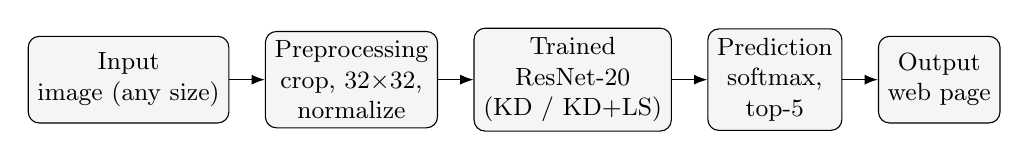
\begin{tikzpicture}[node distance=0.45cm, box/.style={draw,rounded corners,align=center,minimum height=1.1cm,font=\small,fill=gray!8}]
\node[box] (in) {Input\\image (any size)};
\node[box,right=of in] (pre) {Preprocessing\\crop, $32{\times}32$,\\normalize};
\node[box,right=of pre] (m) {Trained\\ResNet-20\\(KD / KD+LS)};
\node[box,right=of m] (p) {Prediction\\softmax,\\top-5};
\node[box,right=of p] (o) {Output\\web page};
\draw[-{Latex}] (in)--(pre); \draw[-{Latex}] (pre)--(m); \draw[-{Latex}] (m)--(p); \draw[-{Latex}] (p)--(o);
\end{tikzpicture}
\end{center}

The pipeline is implemented once in \texttt{lskd/inference.py} and used by both the command-line tool (\texttt{infer.py}) and the Streamlit web app (\texttt{app.py}). Preprocessing is identical to the test-time transform used in evaluation.

\subsection{Starting the application}
\begin{lstlisting}
pip install -r requirements.txt
# put student_kd.pth, student_kd_ls.pth and teachers/resnet56_cifar100.pth in checkpoints/
python scripts/export_demo_images.py      # once: 60 unseen CIFAR-100 test images
streamlit run app.py                      # opens http://localhost:8501
\end{lstlisting}
Dependencies: Python $\geq$3.9, PyTorch, torchvision, NumPy, Pillow, Matplotlib, Streamlit. A GPU is not needed.

\subsection{Input and output format}
\textbf{Input:} one RGB image (PNG/JPG/BMP/WEBP, any resolution) uploaded by the user, or one of 60 CIFAR-100 \emph{test} images that the models never saw during training. Non-square images are centre-cropped, then resized to $32\times32$, scaled to $[0,1]$ and normalized; the tensor fed to the network has shape $(1,3,32,32)$.

\textbf{Output:} for each model (KD student, KD+LS student and optionally the teacher): the predicted class and its probability, a top-5 bar chart, the mean and standard deviation of the raw logits and the inference time; a message saying whether the two students agree (and, for test images, whether each is correct); and a plot of the top-20 raw and Z-scored logits of the three models, which visualises the paper's idea on the current image. The sidebar lists each checkpoint's file, epoch, stored test accuracy and SHA-256 hash, demonstrating that predictions are computed live by the submitted weights.

\subsection{Example inference}
\begin{lstlisting}
$ python infer.py --ckpt checkpoints/student_kd.pth checkpoints/student_kd_ls.pth \
                  --image demo_images/<file>.png
\end{lstlisting}
\TODO{Paste the printed output here (top-5 classes and probabilities for both models).}

\subsection{Screenshots}
\maybefig{screenshots/app_input.png}{Web app: input selection and preprocessing view.}{fig:app1}
\maybefig{screenshots/app_predictions.png}{Web app: predictions of the KD student, KD+LS student and teacher, with raw vs.\ Z-scored logits.}{fig:app2}

% ============================================================
\section{Limitations}
% ============================================================
\begin{itemize}[nosep]
\item \textbf{Statistical power:} one seed per configuration; effects of a few tenths of a point cannot be separated from noise with certainty. The paper averages four runs.
\item \textbf{Scope:} one teacher--student pair on CIFAR-100 (plus CIFAR-10); we did not test ImageNet, different architectures (e.g.\ ResNet32$\times$4$\rightarrow$ShuffleNet), or LS combined with DKD/CTKD/MLKD.
\item \textbf{Self-trained CIFAR-10 teacher:} Experiment B uses a teacher we trained, so its quality may differ from a well-tuned public teacher.
\item \textbf{Test set used for monitoring:} no separate validation split was held out; we mitigate this by reporting final-epoch accuracy and not tuning any hyper-parameter on the test set.
\item \textbf{Deployment domain shift:} the models are trained on $32\times32$ CIFAR images; real photos uploaded in the app are downscaled heavily and differ in style, so accuracy on them is lower than the test accuracy.
\item \textbf{Reduced compute:} mixed precision and GPU-side augmentation are minor deviations from the original implementation.
\end{itemize}

% ============================================================
\section{Conclusion}
% ============================================================
We studied the claim that sharing one temperature between teacher and student in knowledge distillation forces the student to match the teacher's logit magnitude and variance, and that a per-sample Z-score standardization of both logit vectors removes this constraint. We explained the method and its entropy-maximisation motivation in our own words, verified its mathematical properties and the paper's toy example with our own code, and re-implemented and trained vanilla KD and KD+LS for ResNet-56$\rightarrow$ResNet-20 on CIFAR-100, obtaining \KDacc\% and \LSacc\% versus the paper's 70.66\% and 71.43\%. \TODO{One sentence on Experiment A's answer and one on Experiment B's answer.} Finally, we packaged both students in a web application that shows every step from input image to prediction and visualises the difference between raw and standardized logits. Overall, logit standardization is a one-line, parameter-free change that \TODO{did / did not} measurably help in our setting.

% ============================================================
\begin{thebibliography}{99}
% ============================================================
\bibitem{sun2024} S. Sun, W. Ren, J. Li, R. Wang, and X. Cao, ``Logit standardization in knowledge distillation,'' in \textit{Proc. IEEE/CVF Conf. Computer Vision and Pattern Recognition (CVPR)}, 2024, pp. 15731--15740, doi: 10.1109/CVPR52733.2024.01489.
\bibitem{sun2024code} S. Sun, ``logit-standardization-KD,'' GitHub repository, 2024. [Online]. Available: \url{https://github.com/sunshangquan/logit-standardization-KD}
\bibitem{mdistiller} Megvii Research, ``mdistiller: The codebase for knowledge distillation,'' GitHub repository. [Online]. Available: \url{https://github.com/megvii-research/mdistiller}
\bibitem{hinton2015} G. Hinton, O. Vinyals, and J. Dean, ``Distilling the knowledge in a neural network,'' arXiv:1503.02531, 2015.
\bibitem{he2016} K. He, X. Zhang, S. Ren, and J. Sun, ``Deep residual learning for image recognition,'' in \textit{Proc. CVPR}, 2016, pp. 770--778.
\bibitem{krizhevsky2009} A. Krizhevsky, ``Learning multiple layers of features from tiny images,'' Tech. Rep., University of Toronto, 2009.
\bibitem{hu2023} C. Hu \textit{et al.}, ``Teacher-student architecture for knowledge distillation: A survey,'' arXiv:2308.04268, 2023.
\bibitem{mansourian2025} A. M. Mansourian \textit{et al.}, ``A comprehensive survey on knowledge distillation,'' arXiv:2503.12067, 2025.
\bibitem{zhao2022} B. Zhao, Q. Cui, R. Song, Y. Qiu, and J. Liang, ``Decoupled knowledge distillation,'' in \textit{Proc. CVPR}, 2022, pp. 11953--11962.
\bibitem{li2023} Z. Li \textit{et al.}, ``Curriculum temperature for knowledge distillation,'' in \textit{Proc. AAAI}, vol. 37, no. 2, 2023, pp. 1504--1512.
\bibitem{jin2023} Y. Jin, J. Wang, and D. Lin, ``Multi-level logit distillation,'' in \textit{Proc. CVPR}, 2023, pp. 24276--24285.
\bibitem{yang2023} Z. Yang \textit{et al.}, ``From knowledge distillation to self-knowledge distillation: A unified approach with normalized loss and customized soft labels,'' in \textit{Proc. ICCV}, 2023, pp. 17185--17194.
\bibitem{wei2024} S. Wei, C. Luo, and Y. Luo, ``Scale decoupled distillation,'' in \textit{Proc. CVPR}, 2024.
\bibitem{sun2025} W. Sun \textit{et al.}, ``Knowledge distillation with refined logits,'' in \textit{Proc. ICCV}, 2025, pp. 1110--1119.
\bibitem{guo2022} J. Guo, ``Reducing the teacher-student gap via adaptive temperatures,'' 2022.
\bibitem{huang2022} T. Huang, S. You, F. Wang, C. Qian, and C. Xu, ``Knowledge distillation from a stronger teacher,'' in \textit{Advances in Neural Information Processing Systems (NeurIPS)}, 2022.
\bibitem{cho2019} J. H. Cho and B. Hariharan, ``On the efficacy of knowledge distillation,'' in \textit{Proc. ICCV}, 2019.
\bibitem{mirzadeh2020} S. I. Mirzadeh \textit{et al.}, ``Improved knowledge distillation via teacher assistant,'' in \textit{Proc. AAAI}, 2020.
\bibitem{romero2015} A. Romero \textit{et al.}, ``FitNets: Hints for thin deep nets,'' in \textit{Proc. ICLR}, 2015.
\bibitem{tian2020} Y. Tian, D. Krishnan, and P. Isola, ``Contrastive representation distillation,'' in \textit{Proc. ICLR}, 2020.
\bibitem{chen2021} P. Chen, S. Liu, H. Zhao, and J. Jia, ``Distilling knowledge via knowledge review,'' in \textit{Proc. CVPR}, 2021.
\bibitem{park2019} W. Park, D. Kim, Y. Lu, and M. Cho, ``Relational knowledge distillation,'' in \textit{Proc. CVPR}, 2019.
\end{thebibliography}

\appendix
% ============================================================
\section{Summary of revisions from the Mid-Evaluation report}
\label{app:revisions}
\begin{itemize}[nosep]
\item Literature review: condensed the repeated description of the method; added ATKD, the capacity-gap literature and representative feature/relation-based methods (FitNets, CRD, ReviewKD, RKD) that the paper compares against.
\item EDA: added CIFAR-10 split statistics (now used in Experiment B); updated the preprocessing plan to the final pipeline, in which the training-only crop+flip augmentation is enabled.
\item Corrected a team member's name (Bismah Imran) and added all student IDs; fixed duplicate figure labels.
\item Planned experiments: the proposal's ``small temperature study'' became the optional Experiment C; we added the ablation of Experiment A because it addresses a confound (KD weight) that a temperature sweep cannot.
\end{itemize}

\section{All training runs}
\begin{table}[H]
\centering
\caption{Every run used in this report (generated from \texttt{runs/*/summary.json}).}
\small
\begin{tabular}{llcccccc}
\toprule
Run & Method & $T/\tau$ & $\lambda_{KD}$ & Epochs & Final & Best & Minutes \\
\midrule
\gentable{tab_runs}{8}
\bottomrule
\end{tabular}
\end{table}

\section{Use of AI assistance}
\label{app:ai}
\TODO{State honestly how AI tools were used, following the course policy (e.g.\ ``AI assistants were used to help draft code and text; the team ran all experiments, checked all code and results, and is responsible for the content.'')}

\end{document}
